\subsection{y* cut Optimization}
\label{section: y* cut optimization}

In QCD two-to-two scattering, $t$-channel is dominant. The QCD dijet production is proportional to $(1-cos\theta^{*})^{-2}$, while $H'$ and $String$ production is expected to be flat in $cos\theta^{*}$.
This means that $y^{*}$($y^{*} = \frac{y_{1}-y_{2}}{2}$) of QCD background will minimize at 0 and that of $H'$ and $String$ will peak at 0.

Figure \ref{fig: hprime significance as a function of y* cut} shows the significance of $H'$($Significance = \sqrt{\sum_{i}{2\cdot((S_{i}+B_{i})\cdot ln(1+\frac{S_{i}}{B_{i}})-S_{i})}}$) for the $m_{jj}$ distribution as a function of $y^{*}$ cut. The significance peaks at around 0.6, so the optimal $y^{*}$ cut for the $H'$ search is $|y^{*}| < 0.6$.

Figure \ref{fig: string significance as a function of y* cut} shows the significance of $String$ for the $m_{jj}$ distribution as a function of $y^{*}$ cut. The significance peaks at around 0.8, so the optimal $y^{*}$ cut for the $String$ search is $|y^{*}| < 0.8$.

\begin{figure}[htbp]
        \centering
        \subfigure[$\geq$1 g-tag]{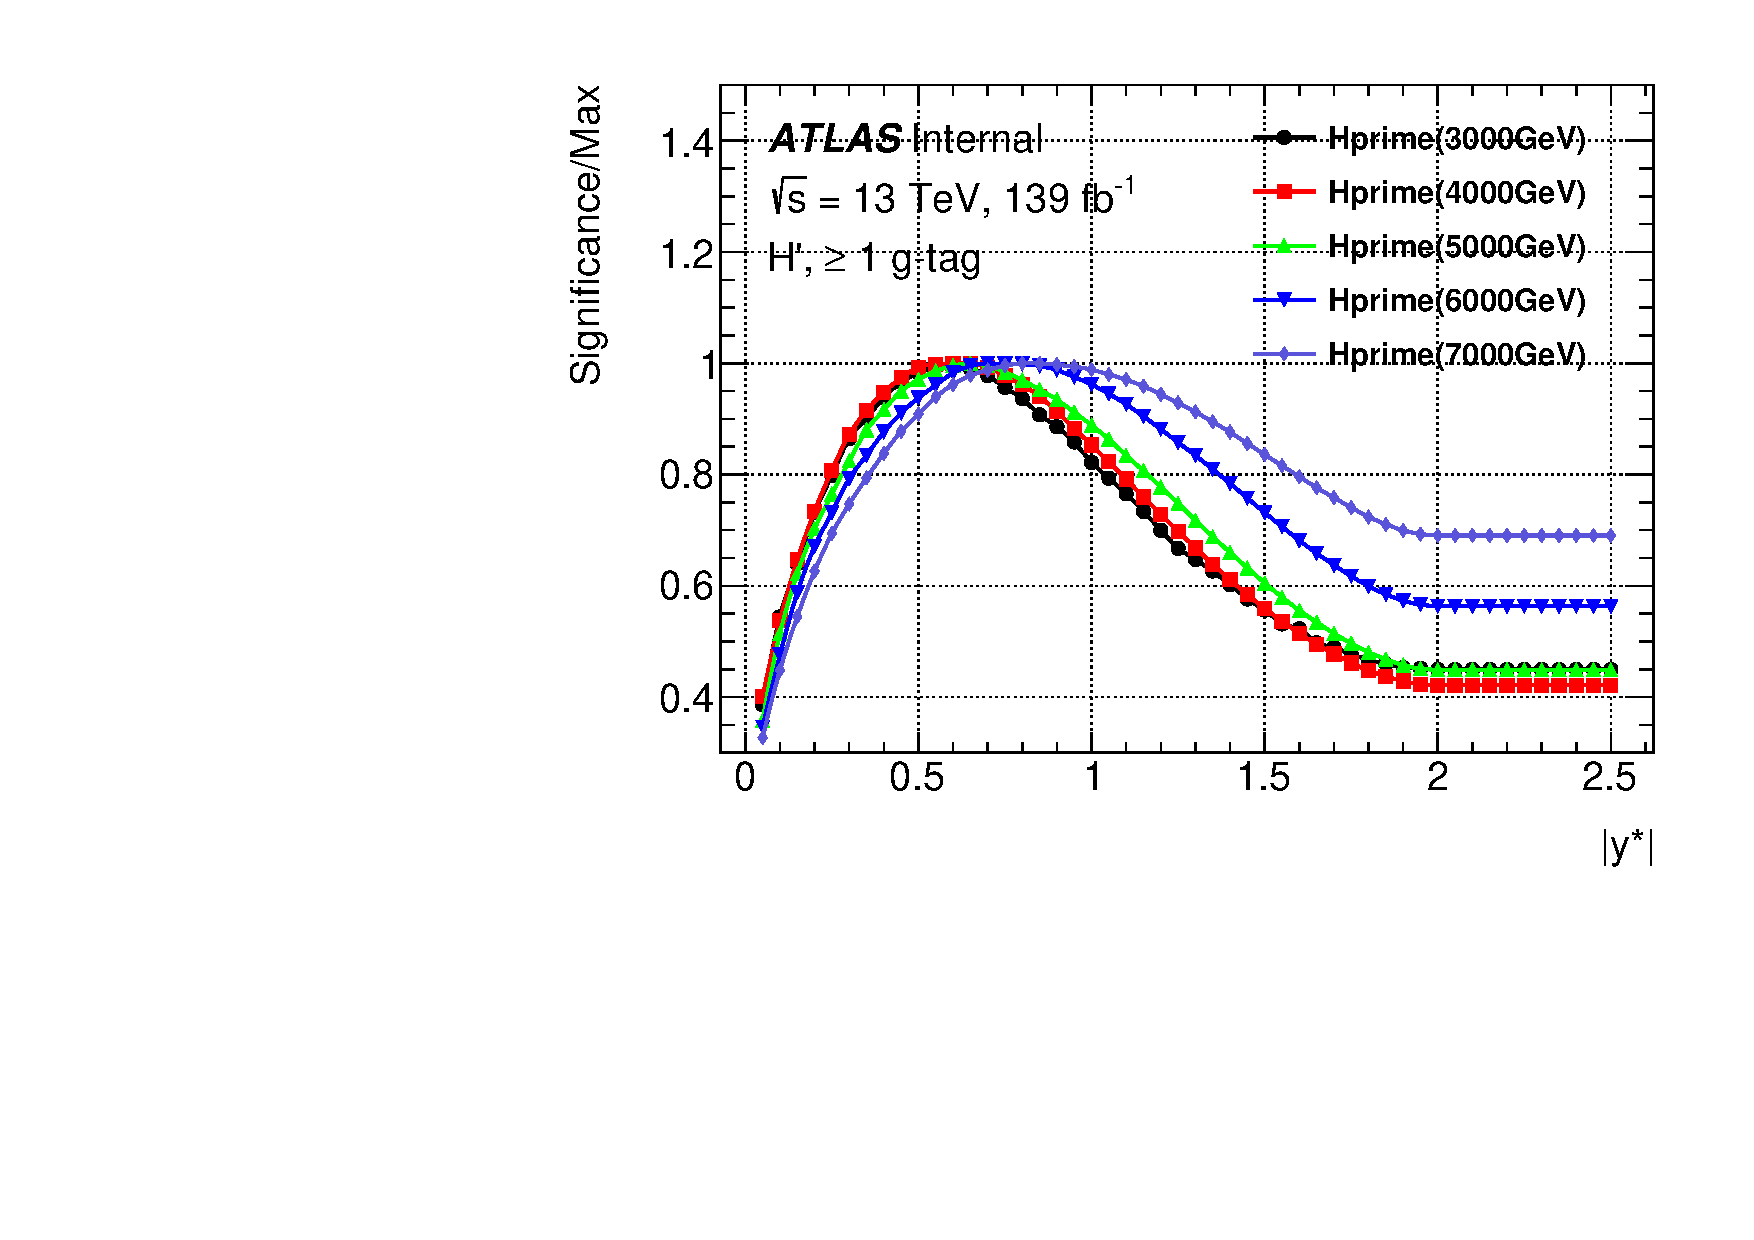
\includegraphics[width=0.48\columnwidth]{figures/yStarOptimization/Significance_Hprime_gj.pdf}}
        \subfigure[2 g-tag]{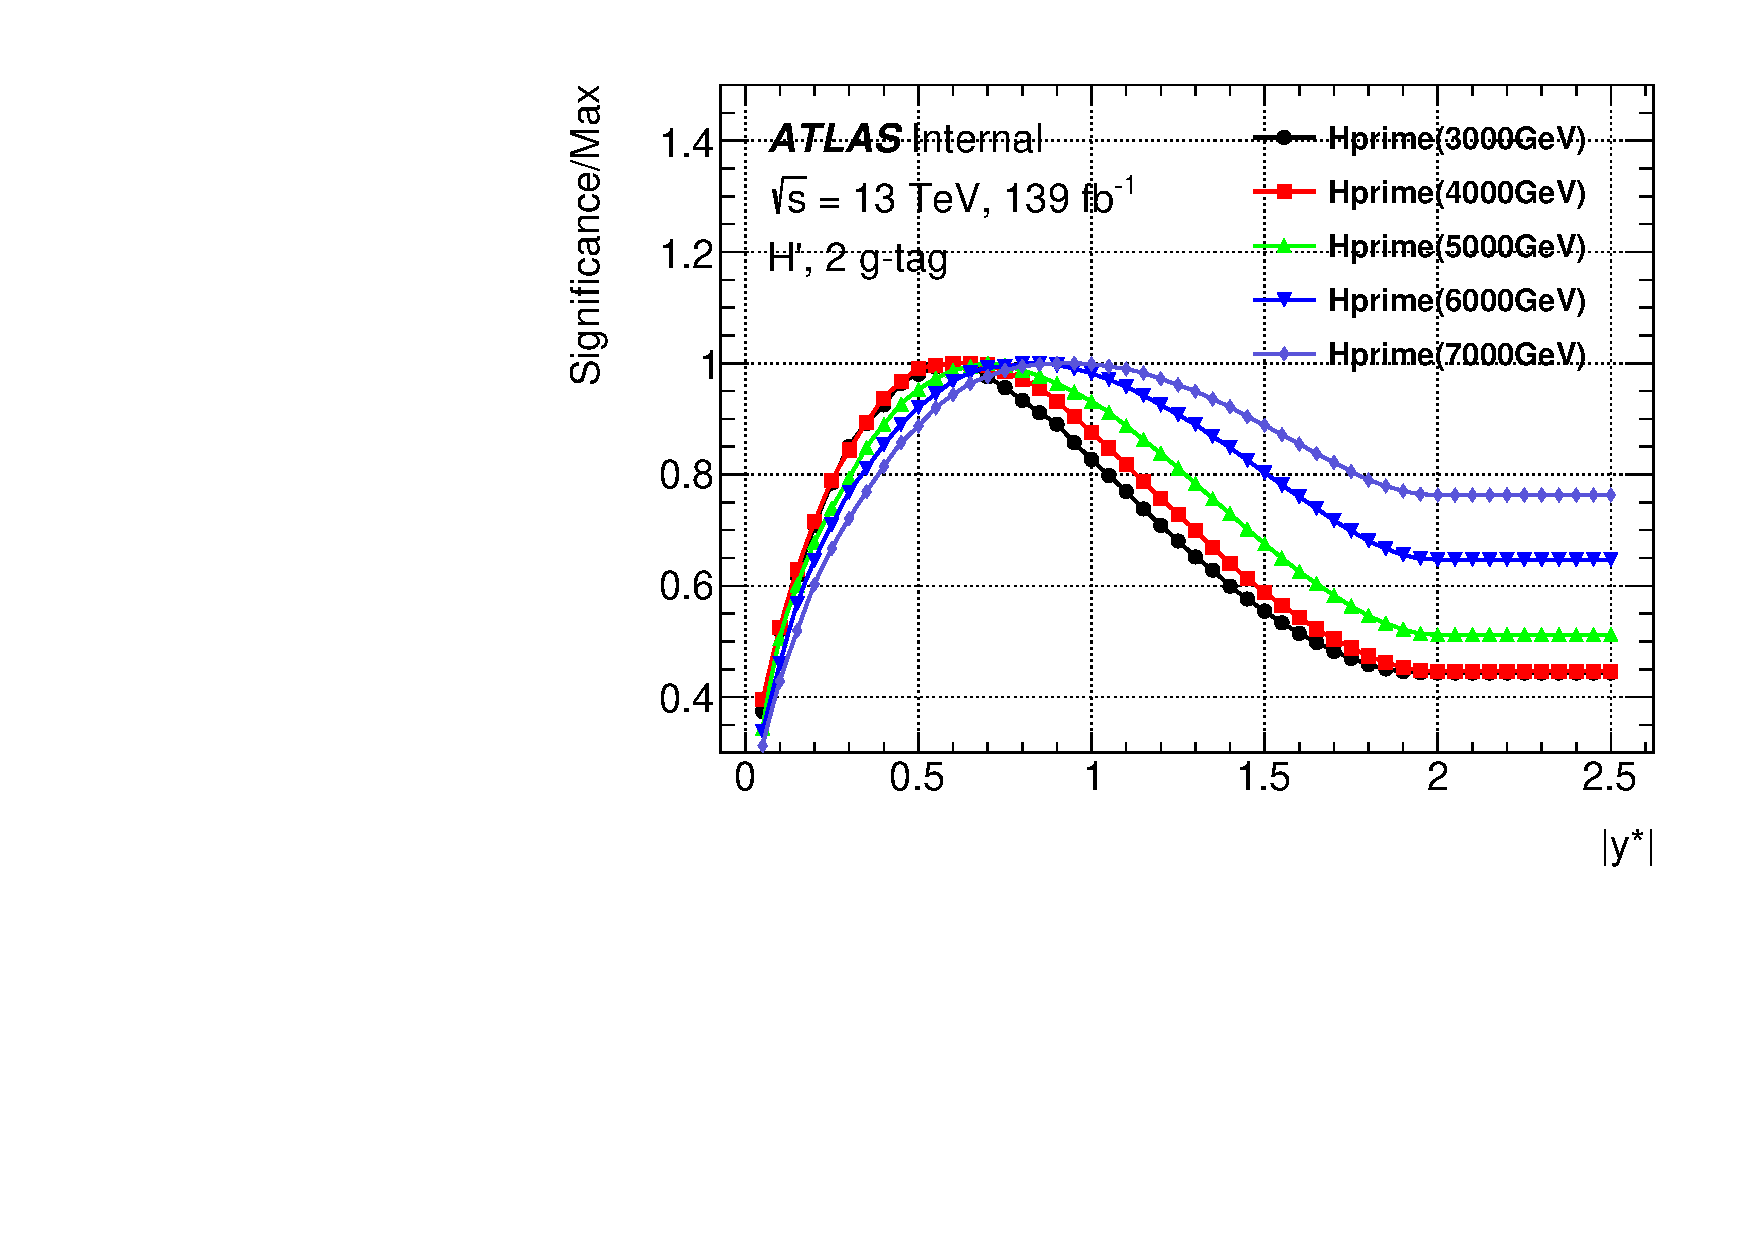
\includegraphics[width=0.48\columnwidth]{figures/yStarOptimization/Significance_Hprime_gg.pdf}}
        \caption{$H'$ significance as a function y* cut in the case of (a) $\geq$1 g-tag, (b) 2 g-tag.}
        \label{fig: hprime significance as a function of y* cut}
\end{figure}


\begin{figure}[htbp]
        \centering
        \subfigure[$\geq$1 g-tag]{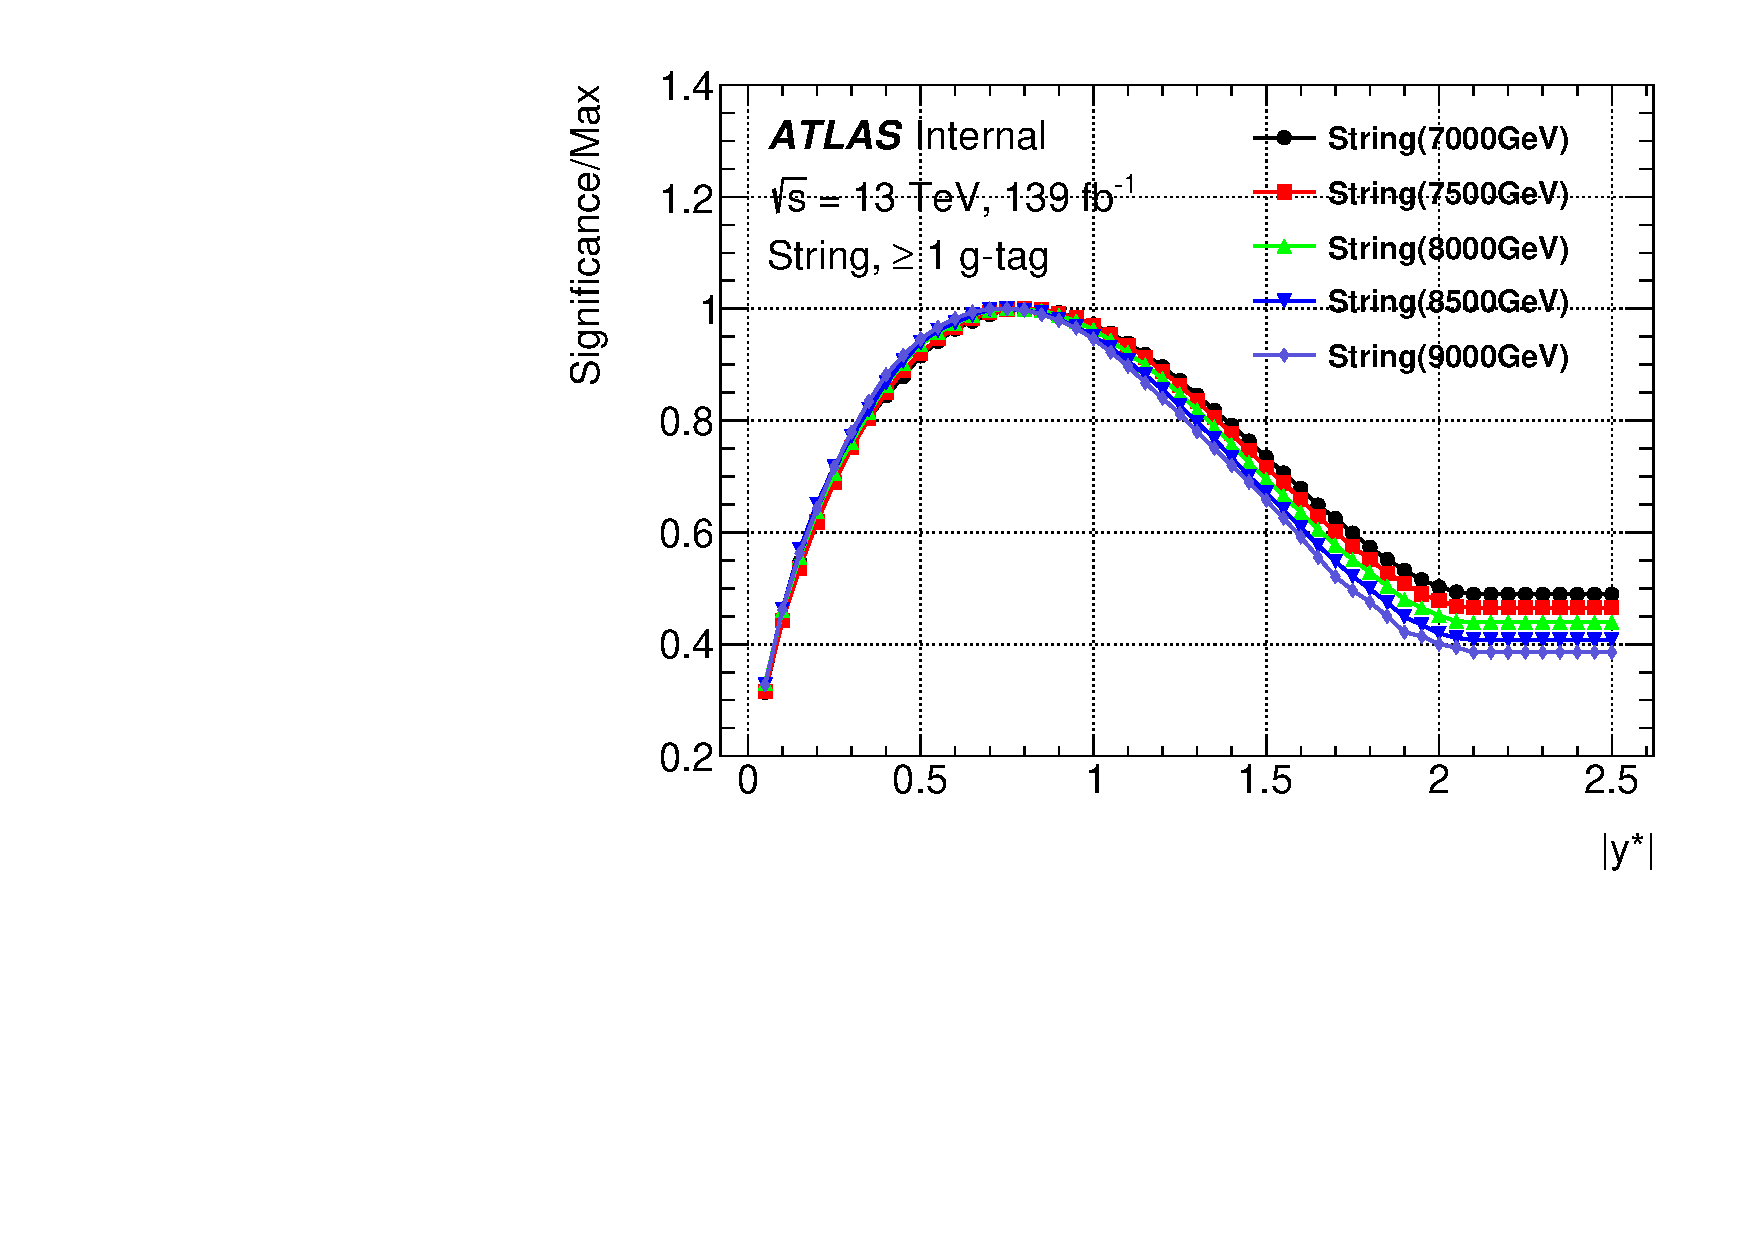
\includegraphics[width=0.48\columnwidth]{figures/yStarOptimization/Significance_String_gj.pdf}}
        \subfigure[2 g-tag]{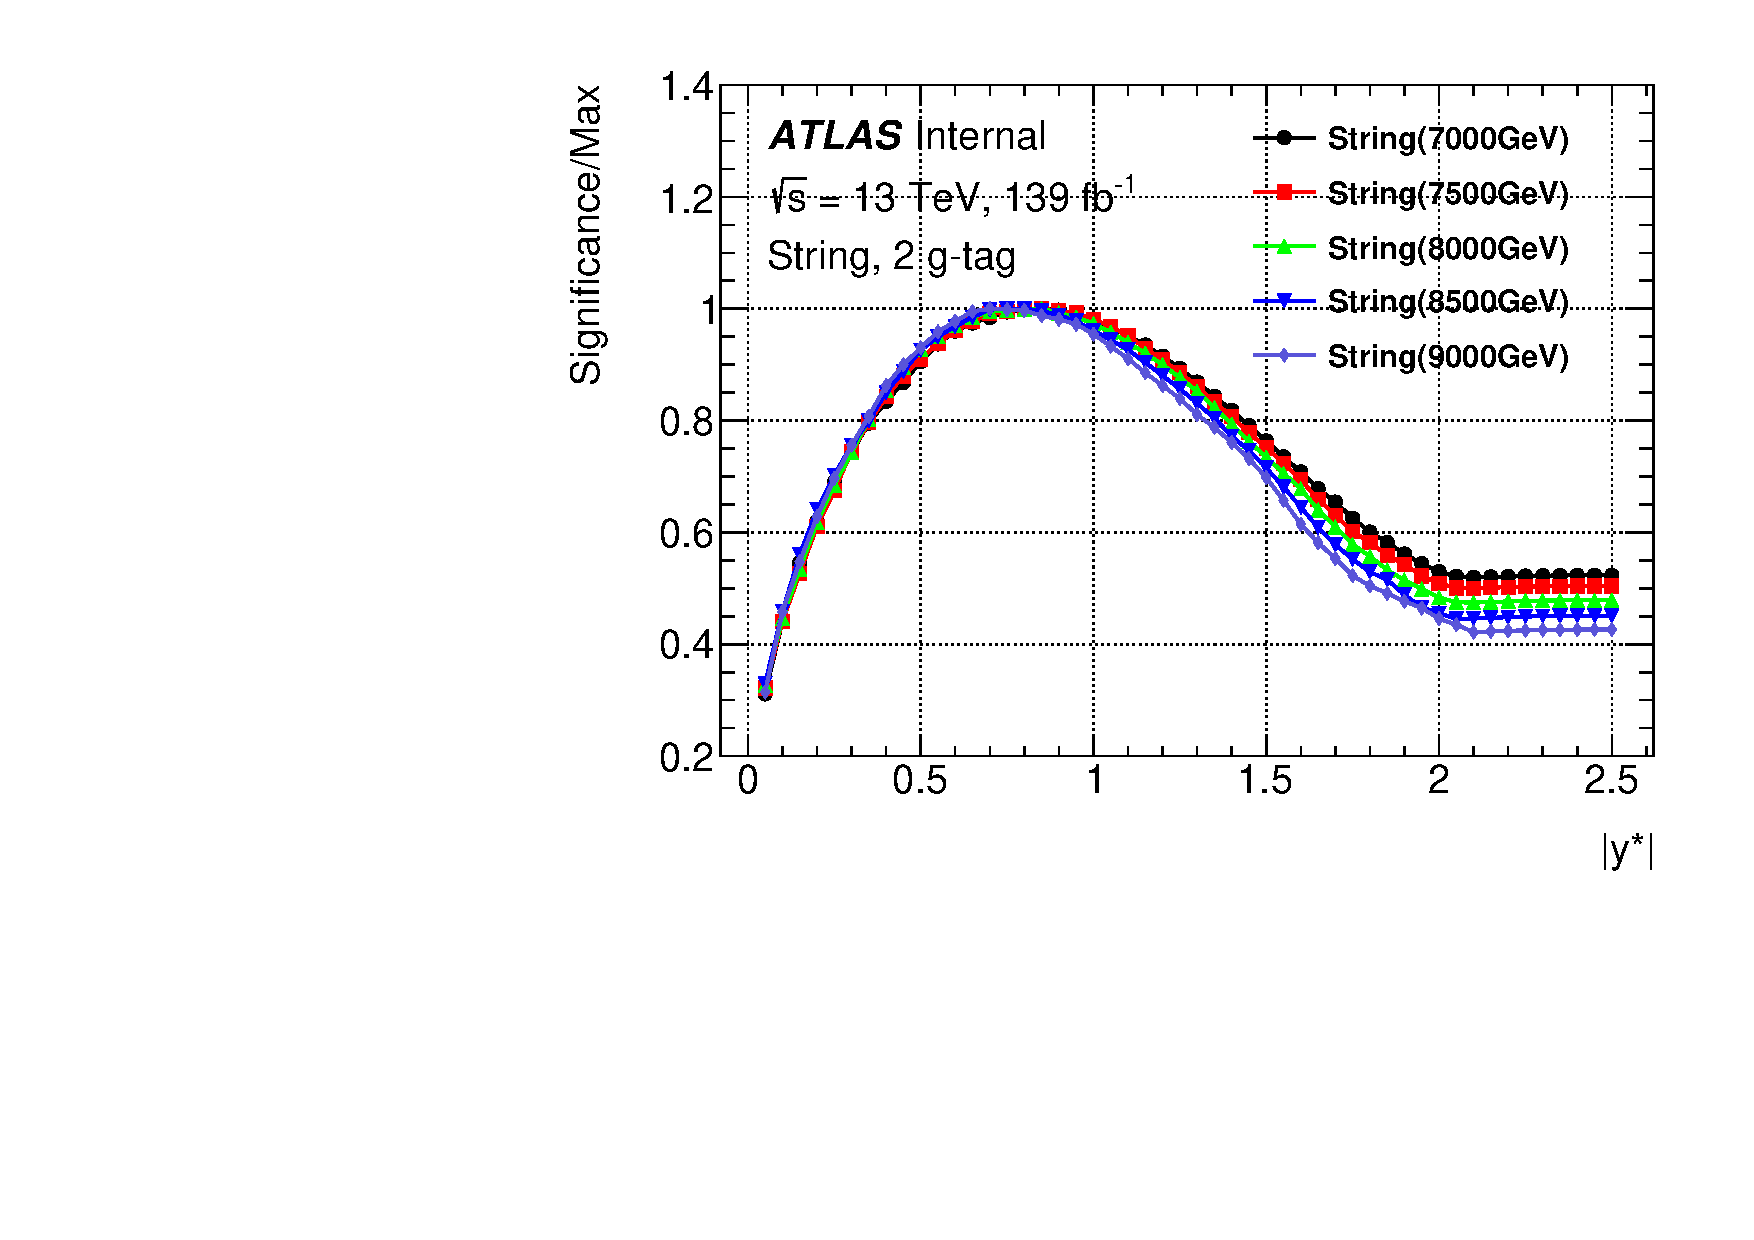
\includegraphics[width=0.48\columnwidth]{figures/yStarOptimization/Significance_String_gg.pdf}}
        \caption{$String$ significance as a function y* cut in the case of (a) $\geq$1 g-tag, (b) 2 g-tag.}
        \label{fig: string significance as a function of y* cut}
\end{figure}
